\documentclass[10pt]{article}
\usepackage[a4paper,margin=20mm,headheight=15pt]{geometry}
\usepackage[T1]{fontenc}
\usepackage{lmodern,microtype}
\usepackage{graphicx,booktabs,longtable,tabularx,array}
\usepackage{xcolor,fancyhdr,hyperref,enumitem}
\usepackage{float}
\definecolor{Ink}{HTML}{172334}
\definecolor{Blue}{HTML}{155E80}
\definecolor{Pale}{HTML}{EAF1F7}
\definecolor{Muted}{HTML}{526172}
\hypersetup{colorlinks=true,urlcolor=Blue,linkcolor=Blue}
\setlength{\parindent}{0pt}
\setlength{\parskip}{4pt}
\setlength{\tabcolsep}{5pt}
\renewcommand{\arraystretch}{1.12}
\setlist[itemize]{topsep=2pt,itemsep=2pt,leftmargin=18pt}
\pagestyle{fancy}\fancyhf{}
\fancyhead[L]{\small\color{Muted}HighamBench / NumStability}
\fancyhead[R]{\small\color{Muted}Observed-use scope analysis, 30 tasks}
\fancyfoot[R]{\small\thepage}
\renewcommand{\headrulewidth}{0.3pt}
\newcommand{\pathref}[1]{\nolinkurl{#1}}
\newcommand{\plot}[1]{\includegraphics[width=0.78\linewidth]{figures/#1.png}}
\newcommand{\ReportTasks}{30}
\newcommand{\ReportPapers}{25}
\newcommand{\ReportPairs}{90}
\newcommand{\ReportAttempts}{180}
\newcommand{\ConsistentUseTasks}{12}
\newcommand{\ZeroUseTasks}{17}
\newcommand{\TimeGainTotals}{+35.0\%}
\newcommand{\TokenGainTotals}{+11.8\%}
\newcommand{\LocGainTotals}{+18.0\%}
\newcommand{\TimeBetterTasks}{23}
\newcommand{\TokenBetterTasks}{20}
\newcommand{\LocBetterTasks}{19}
\newcommand{\ConsistentTimeMean}{+55.8\%}
\newcommand{\ConsistentLocMean}{+43.3\%}
\newcommand{\ZeroTimeMean}{+5.7\%}
\newcommand{\ZeroLocMean}{-1.8\%}

\renewcommand{\LocGainTotals}{+18.3\%}
\renewcommand{\LocBetterTasks}{19}

\newcommand{\DPTimeRho}{+0.69}
\newcommand{\DPCodeRho}{+0.61}
\newcommand{\DPTokenRho}{+0.26}
\newcommand{\DPZeroTasks}{17}
\newcommand{\DPConsistentTasks}{12}


\begin{document}

\begin{center}
{\LARGE\bfseries\color{Ink}NumStability Reuse in a 30-Task HighamBench Scope Analysis}\par
\vspace{3pt}
{\large Protocol, archived proof outcomes, observed declaration use, and comparison with the separate formalize-and-prove benchmark}\par
\vspace{5pt}
{\small 2 October 2026 \quad\textbar\quad \ReportPapers\ paper identifiers \quad\textbar\quad \ReportPairs\ paired repetitions \quad\textbar\quad \ReportAttempts\ accepted attempts}
\end{center}

\colorbox{Pale}{\parbox{0.975\linewidth}{\small
This report is a \emph{post-run scope analysis of archived results}, not a new model run or a prospectively selected independent pilot. It removes every task from six papers after inspection of the earlier full-cohort outcomes and expected-category fit. The full original report, its data, and the prior plot-only scope analysis are preserved separately. All \ReportTasks\ retained tasks, including unfavorable results, appear below.}}

\section*{Abstract}
We examine whether \emph{observed} NumStability use in accepted Lean proofs is associated with lower proof effort on fixed, paper-derived HighamBench targets. Condition N had Lean and Mathlib; condition L additionally had a frozen NumStability snapshot. Each of the \ReportTasks\ retained tasks has three accepted N/L pairs. We recompiled all 90 accepted L proofs under the historical Lean, Mathlib, and NumStability versions and applied the \emph{same direct-proof (DP) scanner} used in the separate ten-task report: distinct library constants in the kernel-accepted proof term and proof-local helper bodies. The task value is the mean of its three counts. Spearman associations with L's time, submitted-code-line, and observed net-new-token gains are respectively $\DPTimeRho$, $\DPCodeRho$, and $\DPTokenRho$. L was faster in \TimeBetterTasks/\ReportTasks\ tasks and submitted fewer nonblank, noncomment lines in \LocBetterTasks/\ReportTasks. Tiers were prior expectations of likely help, not measured use; paper selection was topical rather than random. These descriptive associations are confounded by task and historical campaign, the six-paper scope restriction was chosen after inspecting outcomes, and historical token observations are incomplete lower bounds.\footnote{Primary ledgers: \pathref{../library-usage-analysis/task_usage.csv}, \pathref{../library-usage-analysis/attempt_usage.csv}, and this bundle's \pathref{historical_direct_proof_scan.json}, \pathref{observed_net_new_tokens.json}, \pathref{extended_stats.json}, and \pathref{accepted_code_line_scan.json}. The preserved full-cohort report is \pathref{../usage-without-tiers/report.pdf}, SHA-256 \texttt{27a18f8e9826d5a78b3855faad1b5a6f908b1ada6ff79214c4b0eddef9bf08f9}.}

\section{Question, scope, and provenance}
The question answered is narrow: \emph{when the final accepted L proof actually reaches NumStability declarations, how do N/L elapsed time, observed net-new tokens, and submitted code size compare?} The audit of a proof's dependencies does not measure all useful mathematics available but left undiscovered. It also cannot on its own establish that use caused the gain.

The six omitted paper identifiers are \texttt{P02, P17, P20, P33, P35, P40}; all their archived tasks are omitted, not merely individual repetitions. This rule leaves \ReportTasks\ tasks across \ReportPapers\ papers and \ReportPairs\ complete N/L pairs. It was specified \emph{after} outcomes and expectation-fit had been inspected. The resulting report is therefore a sensitivity/eligibility view, and its associations may be strengthened by that choice. It must not be interpreted as a held-out confirmation. The earlier 38-task report remains the full-archive reference.\footnote{Frozen exclusion list and retained IDs: \pathref{../scope-sensitivity-30/scope_manifest.json} and \pathref{../scope-sensitivity-30/retained_tasks.csv}; the original full report: \pathref{../usage-without-tiers/report.tex}.}

The retained results come from two historical sources: \texttt{results-r11} contributes 12 tasks (36 pairs), while the combined \texttt{results-r09}/\texttt{results-r10} archive contributes 18 tasks (54 pairs). \texttt{r10} replaced infrastructure-affected \texttt{r09} pairs; it is not an additional replicate. All selected tasks have three complete accepted pairs. The known false-target P16-T3 was already outside the original complete-pair cohort, and the older P12-T1 target remains an archived version rather than its later redesigned task.\footnote{Source-campaign descriptions: \pathref{../live-r11/README.md}, \pathref{../combined-r09-r10/README.md}, and \pathref{../../MEASUREMENT_PROGRESS.md}.}

\subsection*{Why these papers and tiers existed}
The paper search followed numerical-stability topics connected to Higham's work and the book's mathematical landscape: floating-point error models, algorithms, perturbation bounds, and stability analyses. It was a purposive topical corpus, not a random sample of all numerical-analysis papers. The source manifest records the selected papers and exact results.\footnote{\pathref{../../metadata/manifest.json}; construction overview and tier definitions in \pathref{../../README.md}.}

The construction aim was to obtain up to three different task types from a paper. An early instruction to find all three types in every paper produced poor-fitting candidates; the later construction rule allowed a tier to be skipped when the paper supplied no suitable source result. T1 anticipated a task that one substantial library result could materially shorten; T2 anticipated combining at least two such results; T3 anticipated comparably demanding mathematics beyond the available library result. These were \emph{pre-run expectations}, informed by the Higham-related subject matter and the task construction review, not labels calculated from the contestant's final declarations. The final rule is documented in the construction README; the account of the earlier forced-three-stage search is the study owner's design history.\footnote{\pathref{../../README.md}, Task types; \pathref{../../metadata/manifest.json}.}

The retained sample has nine T1, three T2, and eighteen T3 tasks: most are in the anticipated low-help tier. Testing whether those expectations match \emph{observed} library use is an analysis outcome, not a premise. A T3 task can still use supporting declarations, and zero final use can reflect failed discovery or an interface mismatch rather than mathematical noncoverage. Because tier and campaign almost coincide here, neither a tier gradient nor a direct-use gradient isolates a causal library effect.\footnote{\pathref{../scope-sensitivity-30/retained_tasks.csv}; \pathref{../library-usage-analysis/attempt_usage.csv}.}

\section{What the archived benchmark measured}
\subsection*{Conditions and fixed target}
This was a \emph{fixed-target proof} study. Both conditions saw the same paper-scoped task context and a fixed Lean theorem signature. The contestant had to retain the target namespace, theorem name, arguments, assumptions, and conclusion, and supply a complete \texttt{Candidate.lean} proof. N had Mathlib, with no NumStability source, compiled objects, or search index. L had the same environment plus read-only NumStability source and compiled modules and a short guide encouraging search and imports. There was no shared, pre-task orientation scout. Final hidden validation rejected \texttt{sorry}, \texttt{admit}, extra axioms, unsafe trust escapes, forbidden imports, and changes to the theorem target. Each condition attempt had fresh agent/workspace state, without cross-task solution sharing.\footnote{Tracked task prompt: \pathref{../../measurement_prompt.md}; L guide: \pathref{../../condition_prompts/L.md}; historical run decisions: \pathref{../../MEASUREMENT_PROGRESS.md}. Current tracked measured-v6 protocol files should not be mistaken for the runtime lock of the older r09/r10 and r11 campaigns.}

The clock ran from authenticated prompt release to authenticated final submission. Intermediate Lean checks chosen by the contestant counted as contestant work; hidden final validation ran afterwards and was logged separately. The per-condition cap was 7,200 seconds with no token ceiling. We rescanned every accepted proof using the ten-task controller's rule for nonblank, noncomment Lean lines. This counts contestant-written helpers and import lines in the submitted file, but not source inside imported libraries. Historical physical-line counts remain a secondary diagnostic. Tokens now follow the ten-task formula: \emph{observed net-new tokens = input tokens $-$ cached input tokens $+$ output tokens}. All 180 selected attempt records contain these fields and match their archived hashes and cached-inclusive totals. The historical logger did not capture unobserved in-flight responses, so these aligned counts remain lower bounds. A passing proof of a supplied Lean statement is \emph{not} a fresh candidate-specific paper-faithfulness audit; source faithfulness belongs to upstream task construction and review.\footnote{Timing and acceptance: \pathref{../live-r11/README.md}, \pathref{../combined-r09-r10/README.md}; accepted proof paths and hashes: \pathref{../library-usage-analysis/attempt_usage.csv}; token derivation and checks: \pathref{token_measurement.py} and \pathref{observed_net_new_tokens.json}; per-file code-line scan: \pathref{accepted_code_line_scan.json}.}

\subsection*{Historical execution differences}
\begin{center}\small
\begin{tabularx}{0.98\linewidth}{@{}p{0.18\linewidth}p{0.38\linewidth}X@{}}\toprule
Aspect & r09/r10 source & r11 source \\\midrule
Campaign role & r09 original, r10 fresh infrastructure-rule replacement; 18 retained tasks & Later campaign; 12 retained completed tasks \\
Formalizer & GPT-5.6 Sol, xhigh & GPT-5.6 Sol, xhigh \\
Agent organization & Measured-v4 permitted root/child agent work & Measured-v5 locked one root and disabled subagents \\
Host execution & Four disjoint four-core, 16-GiB slots; concurrent measured attempts & Four disjoint CPU slots; concurrent attempts also shared provider authentication \\
Limit & 7,200 s per condition, no token cap & 7,200 s per condition, no token cap \\
Interpretation & Infrastructure-rule pair replacement & Different control/context version; not a controlled r09/r10 rerun \\
\bottomrule\end{tabularx}
\end{center}
Historical journals additionally document shared-provider queue/cache interaction and changed model-visible host developer context. A later measured-v6 design serialized provider-active attempts partly for this reason. Combining the archived campaigns is useful for a descriptive inventory, not a clean single-protocol treatment estimate.\footnote{\pathref{../../MEASUREMENT_PROGRESS.md}, including measured-v4/v5/v6 entries.}

\subsection*{Frozen software, host, and parallel work}
The accepted attempt records in both historical sources identify
\texttt{gpt-5.6-sol} at \texttt{xhigh} reasoning. The r11 runtime snapshot
identifies Lean \texttt{v4.29.0-rc3}, Mathlib commit
\texttt{e8ea1afc32790ce1d4e1a4e45cc412ba9388716b}, and the read-only
NumStability commit \texttt{045daf28056a6e4358d5de7c22c7a9d7acc2e80e};
sampled r09 and r11 L attempt records authenticate the same NumStability
commit. The recorded host was a 13th-generation Intel Core i9-13900K with
32 logical CPUs and 94.0 GiB physical RAM. Four disjoint cgroup slots used
CPUs 16--19, 20--23, 24--27, and 28--31, each capped at 16 GiB and no swap.
This describes the archived slots, not a new hardware measurement.
\footnote{\pathref{measurements/runs/results-r11/environment/runtime_snapshot.json},
\pathref{environment/host_at_creation.json}, and
\pathref{environment/resource_slots.json}; r09/r11
\pathref{pairs/*/condition-L/attempt.json} records.}

Parallelism was across condition attempts, not within the r11 contestant:
r11 used one root agent per attempt and forbade subagents; r09/r10 allowed
root/child work. A CPU guard admitted at most four condition attempts
concurrently on these slots. The provider remained a shared external
resource, so disjoint local CPUs and RAM did not guarantee independent
wall times. The historical T1/T2 barrier and the later T2-only stop are
documented in the r11 progress log. No one-time L scout was conducted;
library discovery inside a contestant attempt was included in its clock.
\footnote{\pathref{../../MEASUREMENT_PROGRESS.md},
\pathref{measurements/runs/results-r11/campaign_lock.json}.}

\subsection*{Prompt identity, submission, and validation}
The common instruction was to prove a \emph{fixed} Lean theorem in
\texttt{Candidate.lean}; the condition-specific difference was L's
read-only library mount and lookup guide. The prompt required testing the
complete candidate, preserving the theorem surface, and avoiding
\texttt{sorry}, \texttt{admit}, new axioms, unsafe escapes, and network use.
The current tracked text is in \pathref{measurement_prompt.md} and
\pathref{condition_prompts/L.md}; it documents the instruction design but
must not be substituted for the byte-exact effective prompts of these
older campaigns. Each archived attempt instead records its own prompt
SHA-256, byte count, model, reasoning setting, and prompt-start timestamp.
\footnote{\pathref{measurements/runs/results-r11/pairs/P01-T1-rep-01/condition-N/attempt.json},
\pathref{condition-L/attempt.json}, and the analogous r09/r10 records.}

\begin{center}\small
\begin{tabular}{@{}llrp{0.48\linewidth}@{}}\toprule
Example pair & Condition & Prompt bytes & Archived prompt SHA-256 \\\midrule
r09 P03-T3 rep-01 & N & 4,797 & \texttt{c074108813e8f8aa...} \\
r09 P03-T3 rep-01 & L & 5,271 & \texttt{6dd3aa731d6fcf79...} \\
r11 P01-T1 rep-01 & N & 3,513 & \texttt{0900a30ca7091ebf...} \\
r11 P01-T1 rep-01 & L & 3,987 & \texttt{a8374550a810937b...} \\
\bottomrule\end{tabular}
\end{center}
These are examples, not campaign-wide common prompt hashes:
task-specific context changes the effective bytes. The attempt records
carry the complete hashes. The copied archive does not include a
byte-for-byte prompt-text file for every historical attempt, so this
report documents prompt identity and governing rules rather than claiming
to reproduce all effective prompt bodies.

The contestant clock stopped at authenticated final submission. Hidden
validation then compiled the submitted source in an isolated environment,
checked that the theorem statement matched the frozen target, rejected
forbidden proof escapes, and recorded a complete Lean dependency audit.
The accepted proof bytes and hashes are retained alongside each attempt.
The 180 attempts used in this report passed; proof acceptance is a
kernel-checking result for the supplied Lean target, \emph{not} an
independent audit against paper prose. Private chain-of-thought was not
available; observable command and protocol records should not be called
a full reasoning transcript.
\footnote{\pathref{../library-usage-analysis/attempt_usage.csv};
\pathref{measurements/runs/results-r11/pairs/P01-T1-rep-01/condition-L/attempt.json}
shows the validation fields and
\pathref{hidden_chain_of_thought_available=false}.}

\clearpage
\section{Usage measures and outcome definitions}
The primary measure is \emph{direct proof declaration use} (DP), exactly
the proof-term-and-local-helper definition of the separate ten-task report.
For each accepted L submission we compile the hash-verified source to a
Lean module, inspect the kernel-accepted target proof term, follow
contestant-written helpers in that module, and count distinct constants
whose owning compiled module is NumStability. A declaration counts once
per proof even if it is used repeatedly. We average the three accepted
L counts for each task. Imports or source-text mentions alone do not
count. The N condition had no NumStability modules, so its direct proof
count is zero by design.\footnote{Per-proof names and exact source hashes:
\pathref{historical_direct_proof_scan.json}; pinned input identity:
\pathref{historical_dp_manifest_v2.json}; scanner and runner:
\pathref{design33_proof_dependencies.lean} and
\pathref{rescan_historical_dp.py}.}

The rescan used the archived NumStability commit
\texttt{045daf28056a6e4358d5de7c22c7a9d7acc2e80e}, Mathlib commit
\texttt{e8ea1afc32790ce1d4e1a4e45cc412ba9388716b}, and Lean
\texttt{v4.29.0-rc3}. Its manifest verifies every accepted proof and
attempt hash and the historical common-definition source hash before
recompilation. A parallel diagnostic pass had a Lean crash and also
exposed a nonhistorical P09 convenience definition; neither pass feeds
the reported count. The completed final pass uses the campaign-manifest
P09 definition and single-job proof compilation. The old distance-one
target count remains a secondary metric in Appendix~\ref{app:otherusage}.
Unlike DP, it misses library calls hidden behind contestant-written
helpers: P15-T3 has zero distance-one target reach but nonzero direct
proof-helper use in all three accepted L proofs. This fixed-target
experiment has no candidate-formalization phase, so its DP count is
proof-only; the newer study additionally records statement use (DS) and
the statement/proof union (DU). The usage \emph{definition} is now
aligned, but tasks, models, clocks, and protocols remain different.

For a repetition, a positive gain means L used less of the metric: $(N-L)/N\times100\%$. For the task ledger, we first average three N and three L measurements, then compute the gain from those means. Grouped means average task percentages equally. The aggregate table reports the ratio of task-mean totals, which is a different weighting. The main submitted-code metric now uses the ten-task controller's same nonblank, noncomment Lean-line rule on every hash-verified accepted file. Its \emph{surface} still differs: this older task had a fixed statement and one submitted proof file, while the newer task has separately generated statement and proof artifacts. Because the theorem was already fixed, this study has a single proof clock and cannot isolate candidate-formalization from proof time.\footnote{Per-attempt line scan: \pathref{accepted_code_line_scan.json}; exact algorithm: \pathref{make_extended_assets.py}.}

\begin{center}\small
\begin{tabular}{@{}lrrrlrl@{}}\toprule
Metric across \ReportTasks\ task means & N mean & L mean & Gain of totals & L better & Unit & Qualification \\\midrule
Elapsed time & 792.2 & 515.1 & +35.0\% & 23/30 & seconds & mixed historical protocols \\
Observed net-new tokens & 0.109M & 0.097M & +11.8\% & 20/30 & tokens & incomplete lower bounds \\
Submitted code lines & 398.1 & 325.1 & +18.3\% & 19/30 & lines & blank/comment-only excluded \\
\bottomrule

\end{tabular}
\end{center}
The token direction is displayed for completeness, but the 180 historical records cover completed provider responses only; they do not establish exact total spending. Neither the aggregate gains nor grouped task averages should be treated as randomized causal effects.

\begin{figure}[H]\centering
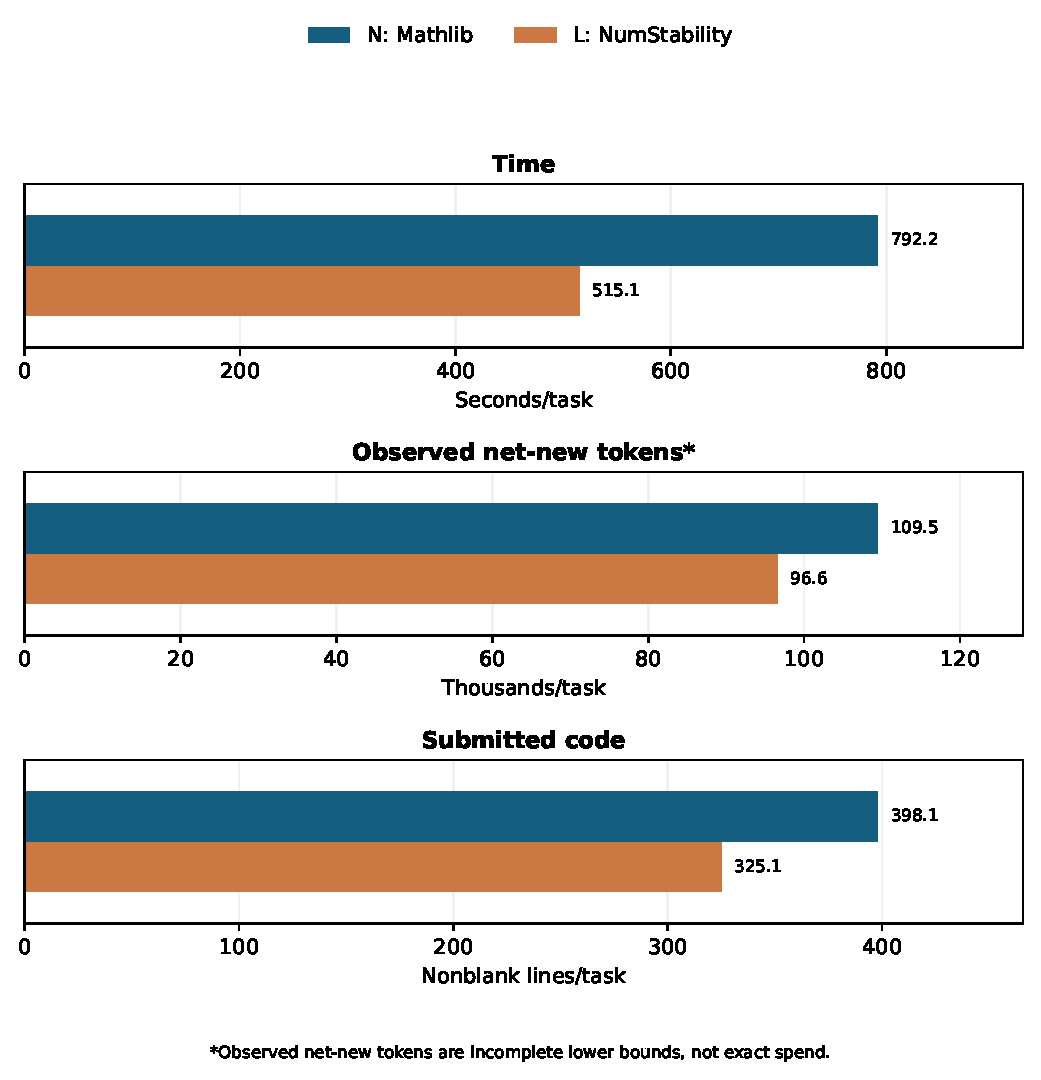
\includegraphics[width=0.82\linewidth]{figures/averages_nl.pdf}
\caption{Absolute N and L arithmetic means per task for the three recorded
proof-task resources, following the paired-value presentation of the
ten-task report. The token comparison uses the same net-new formula,
but incomplete historical observations; it is not an exact token-saving estimate.
Generated from the archived 30-task ledger by
\pathref{make_extended_assets.py}.}
\label{fig:aggregate}
\end{figure}

The target \emph{proof region} can also be counted separately from all
submitted source. Its three-run task-mean average was 94.0 nonblank,
non-comment lines for N and 102.5 for L, a $-9.0\%$ L gain by the
ratio-of-totals convention. This does not contradict the positive
full-file code-line result: helper lemmas before the target are excluded
from the proof-region count, and those helpers can contain much of the
actual work. For code-effort comparisons we therefore retain complete
submitted-file code lines as primary and provide proof-region and historical
physical-line counts only as diagnostics in Appendix~\ref{app:proofregion}.
\footnote{\pathref{../library-usage-analysis/attempt_usage.csv};
\pathref{make_extended_assets.py} and \pathref{extended_stats.json}.}

\clearpage
\section{Library usage and outcomes}
The primary DP count has positive pooled rank associations with all
three recorded proof-task gains. A point is one task, not one repetition;
the horizontal coordinate averages the three final accepted L proof-term
and local-helper counts, and the vertical coordinate is the N-to-L gain
of the three-run task means. The token association concerns incomplete
observed net-new counts.\footnote{\pathref{historical_direct_proof_scan.json};
\pathref{make_extended_assets.py} and \pathref{extended_stats.json}.}

\begin{center}\small
\begin{tabular}{@{}lrrr@{}}\toprule
Use measure & Time $\rho$ & Code lines $\rho$ & Net-new tokens $\rho$\\\midrule
Direct proof declaration use (DP) & +0.69 & +0.61 & +0.26 \\
\bottomrule

\end{tabular}
\end{center}

\begin{figure}[H]\centering
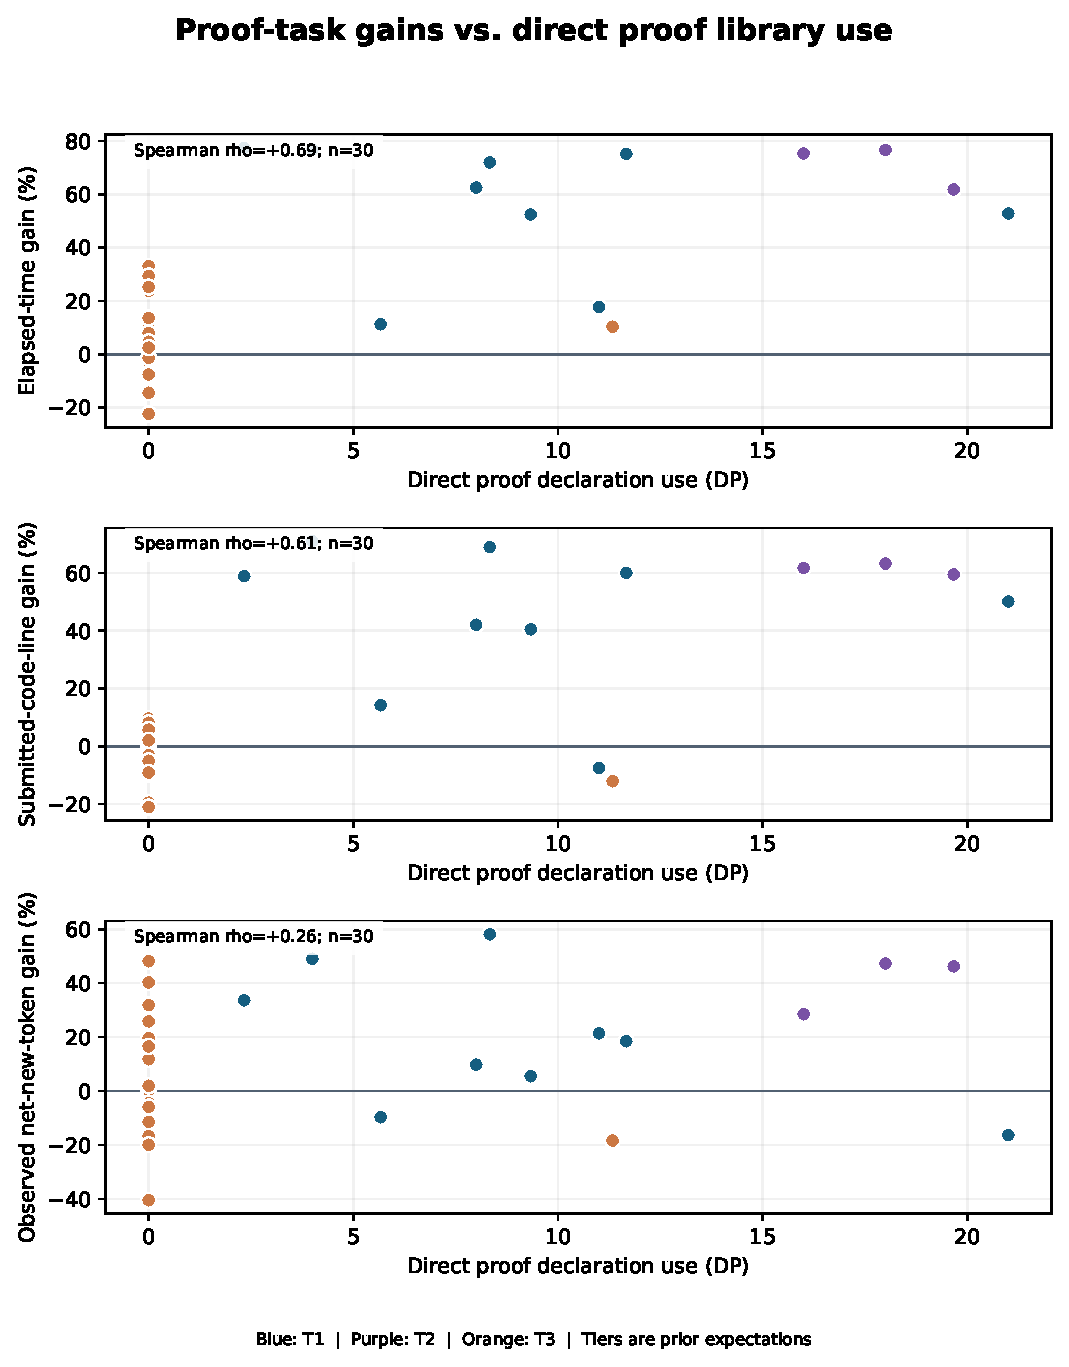
\includegraphics[width=\linewidth]{figures/direct_usage_gains.pdf}
\caption{Direct proof declaration use (DP) versus time,
nonblank submitted code lines, and incomplete observed net-new-token gains.
The horizontal count is the three-run mean number of distinct
NumStability constants in accepted proof terms and contestant-local
helper bodies---the same DP definition as in the ten-task report.
Positive gain favors L. T1/T2/T3 colors show prior expected help, not
a computed use class. The pooled associations are descriptive: direct
use was chosen during the run and tier nearly coincides with campaign.
\pathref{make_extended_assets.py}; \pathref{extended_stats.json}.}
\label{fig:direct}
\end{figure}

The figure is consistent with greater observed DP use accompanying larger
time and complete-code gains in this retained sample. It does not
establish a monotone effect of adding declarations. Task difficulty,
interface fit, discovery, and historical control changes can affect both
use and outcomes. P15-T3 is a particularly important exception to
interpreting a target-only dependency count as all assistance: its
distance-one target count is zero, but DP sees its helper-body use.

\subsection*{Prior tier expectations versus observed direct proof use}
\begin{center}\small
\begin{tabular}{@{}lrrr@{}}\toprule
Expected tier & Tasks & Mean DP count & Tasks with zero DP\\\midrule
T1 & 9 & 9.0 & 0 \\
T2 & 3 & 17.9 & 0 \\
T3 & 18 & 0.6 & 17 \\
\bottomrule

\end{tabular}
\end{center}
The tier table compares prior expectations with \emph{observed} DP use.
The three T2 tasks show extensive direct proof use; T1 is more mixed;
P15-T3 is an important T3 exception, with direct helper-body library use
in all three L proofs. Thus the ordering can be informative in aggregate
without validating each task label. Moreover T1/T2 and T3 came from different
historical campaigns, so the tier comparison is confounded.

\section{Task-level proof-effort comparisons}
Figures~\ref{fig:tasktime}--\ref{fig:taskloc} show the N and L
three-run means directly for every retained task, on a common scale within
each resource. Blue denotes N and orange denotes L throughout, as in the
ten-task report. A shorter L bar is favorable; percentage gains remain in
the numeric ledger and the library-use association plot rather than
replacing the underlying values. The token panel compares incomplete
observed net-new records, not exact usage. This fixed-target benchmark has no
formalization-stage or warm-start measurements to plot.\footnote{\pathref{../library-usage-analysis/task_usage.csv};
\pathref{make_extended_assets.py}.}

\begin{figure}[p]\centering
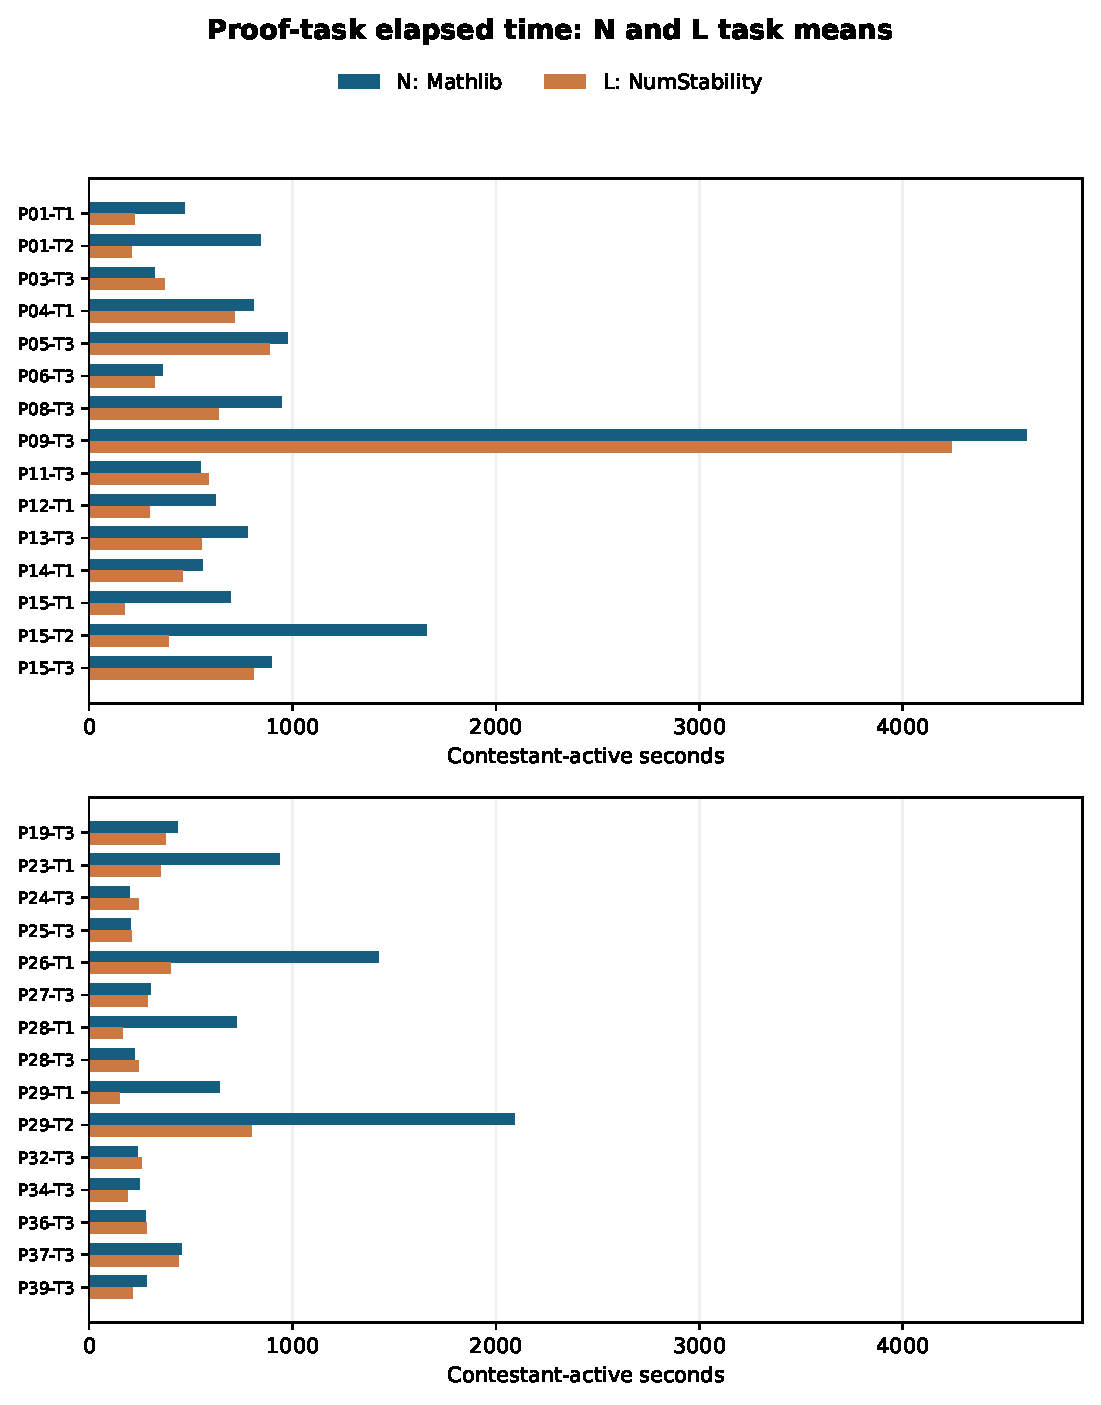
\includegraphics[width=\linewidth,height=.77\textheight,keepaspectratio]{figures/task_time_nl.pdf}
\caption{N and L contestant-active elapsed seconds per task, from
authenticated prompt release to final contestant submission. Each bar
is the mean of three accepted repetitions; there is no separate
formalization/proof-stage split in this fixed-target study.}
\label{fig:tasktime}
\end{figure}
\begin{figure}[p]\centering
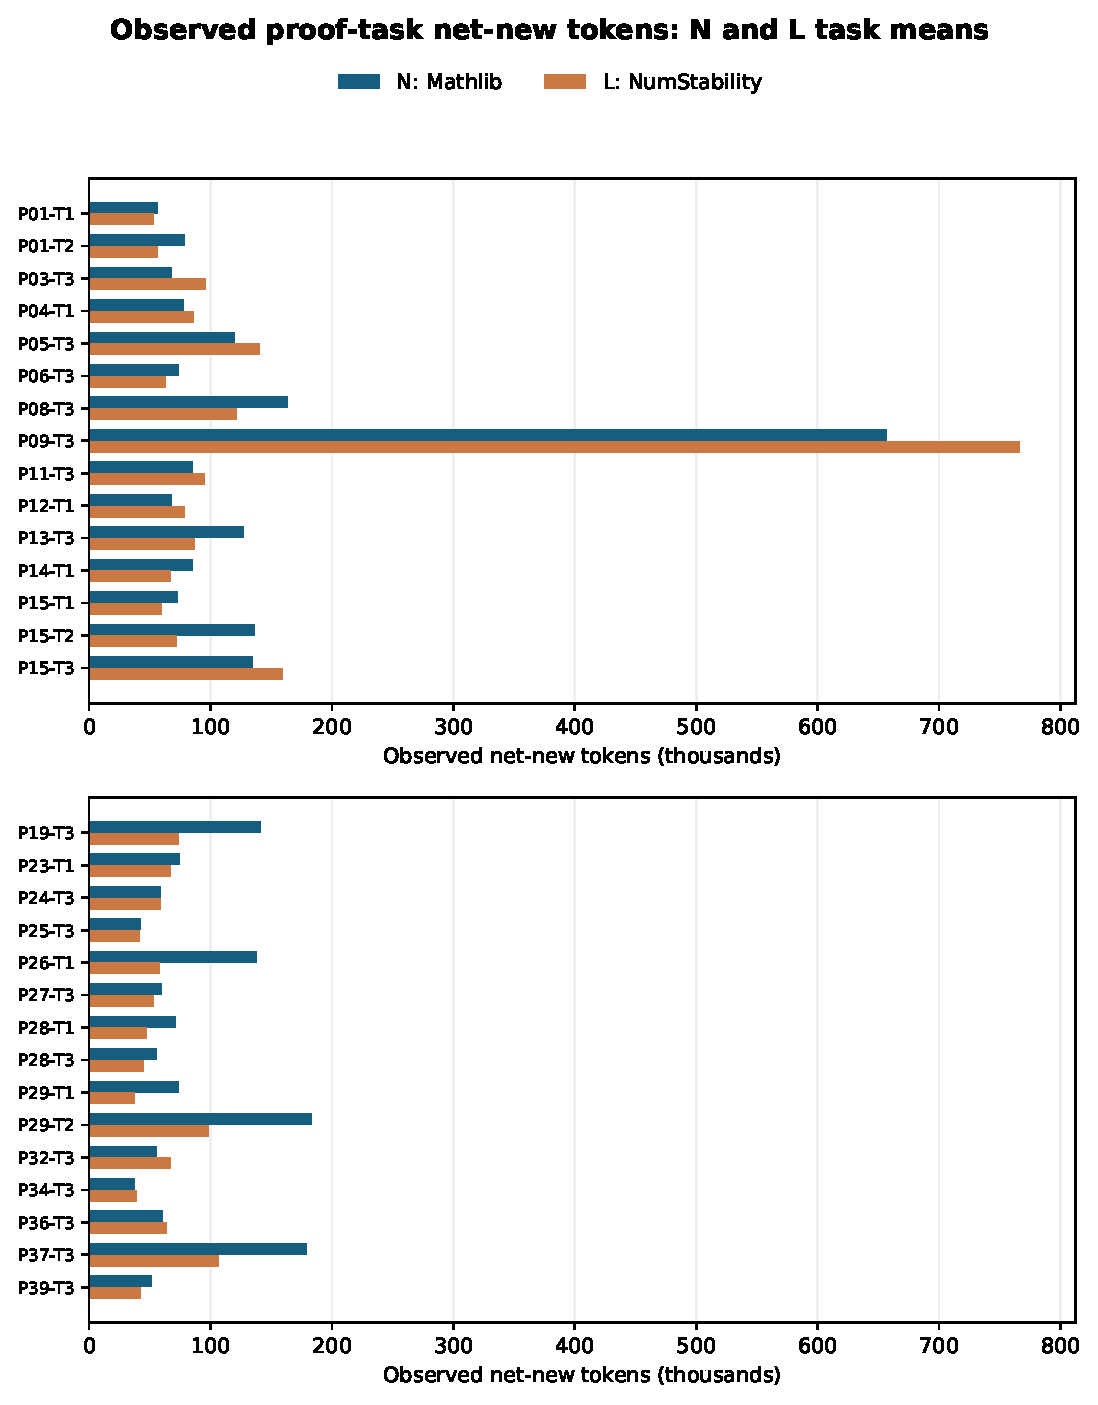
\includegraphics[width=\linewidth,height=.77\textheight,keepaspectratio]{figures/task_tokens_nl.pdf}
\caption{N and L observed net-new tokens per task, in thousands.
Cached input has been subtracted. Unobserved in-flight use prevents
exact total-expenditure claims.}
\label{fig:tasktokens}
\end{figure}
\begin{figure}[p]\centering
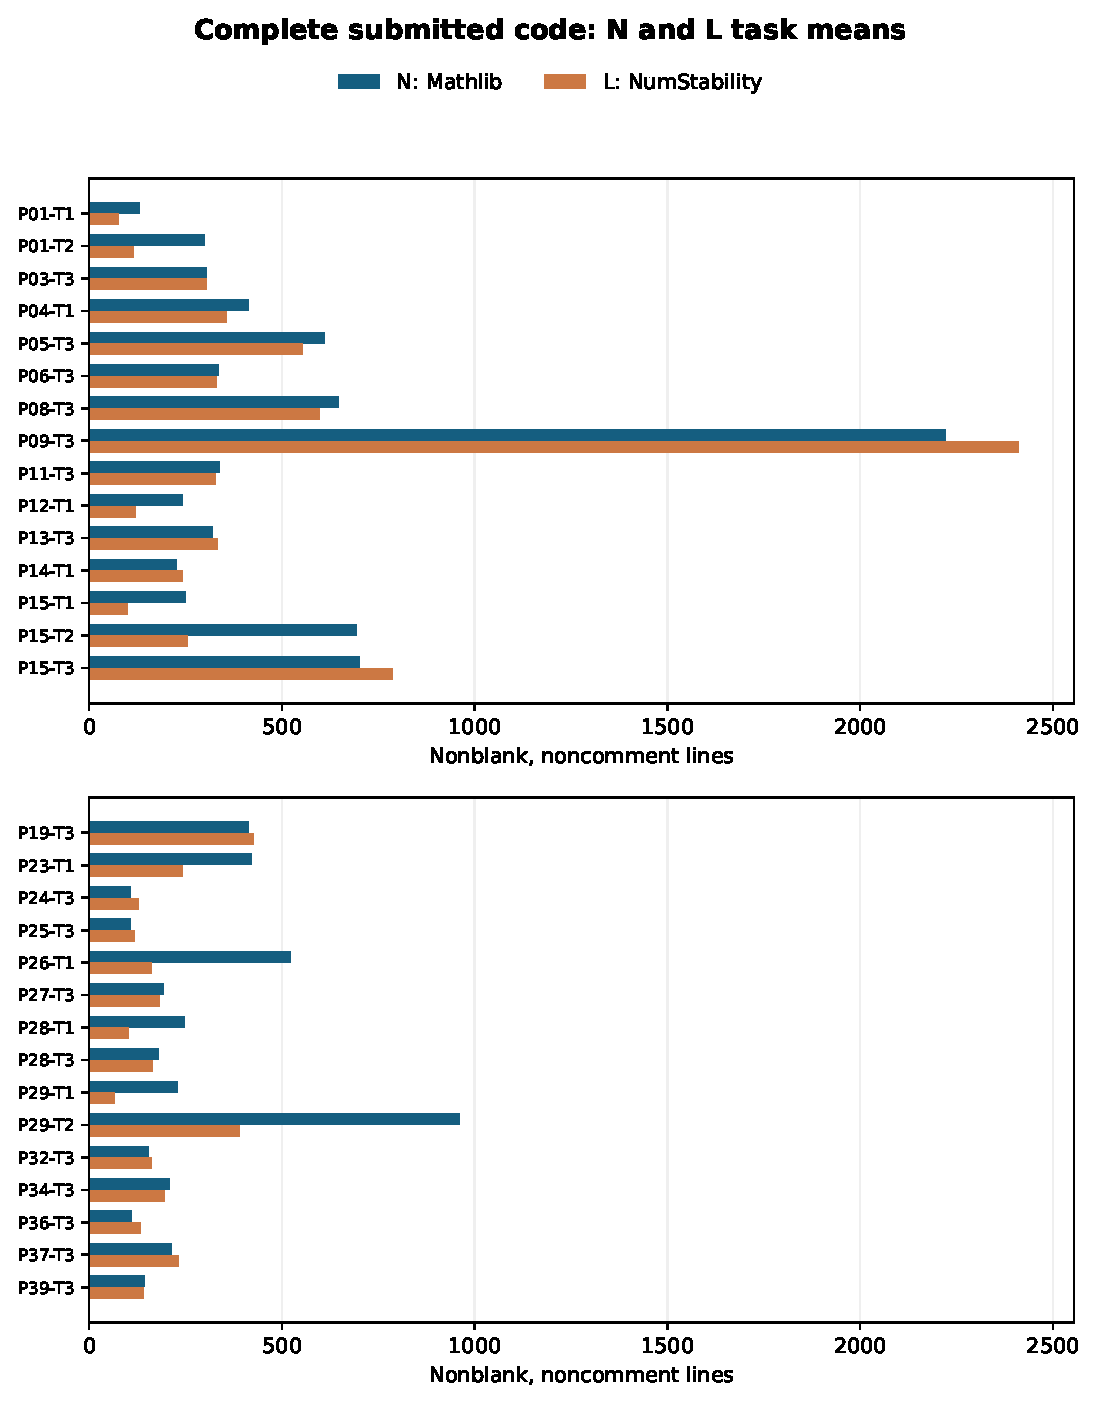
\includegraphics[width=\linewidth,height=.77\textheight,keepaspectratio]{figures/task_loc_nl.pdf}
\caption{N and L nonblank, noncomment lines in complete submitted
proof files. These include contestant-written helpers and import lines,
but not source inside imported libraries. The same lexical line-counting
rule is used in the ten-task report.}
\label{fig:taskloc}
\end{figure}

\clearpage
\section{Complete retained task ledger}
Every retained task is shown, including negative outcomes. The first
table gives raw N/L time and net-new-token values, not only gains; token values
are incomplete observed thousands. The second gives \emph{direct proof
declaration use (DP)}, the mean distinct proof-term/local-helper count across three accepted L
proofs, and the hash-verified nonblank code-line counts. All values are
three-run task means. The historical candidate-list hit measure is not
used as actual library assistance.

\footnotesize\setlength{\tabcolsep}{4pt}\renewcommand{\arraystretch}{1.0}
\begin{longtable}{@{}lrrrrrr@{}}
\caption{Per-task time (seconds) and observed net-new tokens (thousands); positive gain favors L.}\label{tab:resources}\\
\toprule
Task & N time & L time & Time gain & N tokens & L tokens & Token gain \\\midrule
\endfirsthead
\toprule
Task & N time & L time & Time gain & N tokens & L tokens & Token gain \\\midrule
\endhead
P01-T1 & 470 & 224 & +52.4\% & 56 & 53 & +5.5\% \\
P01-T2 & 841 & 208 & +75.3\% & 78 & 56 & +28.5\% \\
P03-T3 & 322 & 369 & -14.5\% & 68 & 96 & -40.5\% \\
P04-T1 & 807 & 716 & +11.2\% & 78 & 86 & -9.7\% \\
P05-T3 & 975 & 888 & +9.0\% & 120 & 140 & -17.1\% \\
P06-T3 & 363 & 321 & +11.6\% & 73 & 63 & +13.9\% \\
P08-T3 & 947 & 635 & +33.0\% & 164 & 121 & +25.8\% \\
P09-T3 & 4608 & 4242 & +7.9\% & 657 & 766 & -16.7\% \\
P11-T3 & 547 & 586 & -7.1\% & 85 & 95 & -11.4\% \\
P12-T1 & 623 & 294 & +52.8\% & 67 & 78 & -16.3\% \\
P13-T3 & 779 & 550 & +29.4\% & 127 & 87 & +31.9\% \\
P14-T1 & 559 & 460 & +17.7\% & 85 & 67 & +21.3\% \\
P15-T1 & 694 & 173 & +75.1\% & 73 & 59 & +18.5\% \\
P15-T2 & 1661 & 389 & +76.6\% & 136 & 72 & +47.3\% \\
P15-T3 & 899 & 806 & +10.3\% & 135 & 160 & -18.4\% \\
P19-T3 & 433 & 374 & +13.6\% & 141 & 73 & +48.1\% \\
P23-T1 & 937 & 351 & +62.5\% & 74 & 67 & +9.8\% \\
P24-T3 & 196 & 240 & -22.4\% & 59 & 59 & +0.3\% \\
P25-T3 & 203 & 208 & -2.6\% & 42 & 41 & +1.9\% \\
P26-T1 & 1423 & 399 & +71.9\% & 138 & 58 & +58.1\% \\
P27-T3 & 301 & 287 & +4.6\% & 60 & 53 & +11.8\% \\
P28-T1 & 726 & 165 & +77.3\% & 71 & 47 & +33.6\% \\
P28-T3 & 225 & 242 & -7.9\% & 56 & 45 & +19.6\% \\
P29-T1 & 641 & 149 & +76.8\% & 73 & 37 & +49.0\% \\
P29-T2 & 2092 & 799 & +61.8\% & 183 & 98 & +46.2\% \\
P32-T3 & 237 & 255 & -7.6\% & 56 & 67 & -19.9\% \\
P34-T3 & 248 & 189 & +23.8\% & 38 & 39 & -4.5\% \\
P36-T3 & 276 & 280 & -1.4\% & 60 & 64 & -5.9\% \\
P37-T3 & 453 & 442 & +2.4\% & 179 & 107 & +40.3\% \\
P39-T3 & 282 & 211 & +25.2\% & 51 & 43 & +16.5\% \\
\bottomrule

\end{longtable}

\begin{longtable}{@{}llrrrr@{}}
\caption{Per-task tier, direct proof declaration use, and nonblank submitted code lines.}\label{tab:tasks}\\
\toprule
Task & Tier & Mean DP & N lines & L lines & Line gain \\\midrule
\endfirsthead
\toprule
Task & Tier & Mean DP & N lines & L lines & Line gain \\\midrule
\endhead
P01-T1 & T1 & 9.3 & 130.0 & 77.3 & +40.5\% \\
P01-T2 & T2 & 16.0 & 298.0 & 114.0 & +61.7\% \\
P03-T3 & T3 & 0.0 & 303.3 & 304.3 & -0.3\% \\
P04-T1 & T1 & 5.7 & 414.3 & 355.3 & +14.2\% \\
P05-T3 & T3 & 0.0 & 611.7 & 552.7 & +9.6\% \\
P06-T3 & T3 & 0.0 & 334.3 & 329.7 & +1.4\% \\
P08-T3 & T3 & 0.0 & 648.0 & 597.7 & +7.8\% \\
P09-T3 & T3 & 0.0 & 2222.3 & 2410.3 & -8.5\% \\
P11-T3 & T3 & 0.0 & 338.0 & 329.0 & +2.7\% \\
P12-T1 & T1 & 21.0 & 243.3 & 121.3 & +50.1\% \\
P13-T3 & T3 & 0.0 & 319.7 & 332.0 & -3.9\% \\
P14-T1 & T1 & 11.0 & 226.0 & 243.0 & -7.5\% \\
P15-T1 & T1 & 11.7 & 249.3 & 99.7 & +60.0\% \\
P15-T2 & T2 & 18.0 & 694.0 & 255.0 & +63.3\% \\
P15-T3 & T3 & 11.3 & 701.3 & 786.0 & -12.1\% \\
P19-T3 & T3 & 0.0 & 413.7 & 426.3 & -3.1\% \\
P23-T1 & T1 & 8.0 & 420.0 & 243.3 & +42.1\% \\
P24-T3 & T3 & 0.0 & 107.7 & 128.7 & -19.5\% \\
P25-T3 & T3 & 0.0 & 107.7 & 118.0 & -9.6\% \\
P26-T1 & T1 & 8.3 & 523.3 & 162.3 & +69.0\% \\
P27-T3 & T3 & 0.0 & 191.7 & 182.3 & +4.9\% \\
P28-T1 & T1 & 2.3 & 248.3 & 102.0 & +58.9\% \\
P28-T3 & T3 & 0.0 & 179.7 & 165.0 & +8.2\% \\
P29-T1 & T1 & 4.0 & 229.0 & 66.3 & +71.0\% \\
P29-T2 & T2 & 19.7 & 961.0 & 389.0 & +59.5\% \\
P32-T3 & T3 & 0.0 & 153.0 & 160.7 & -5.0\% \\
P34-T3 & T3 & 0.0 & 207.7 & 195.7 & +5.8\% \\
P36-T3 & T3 & 0.0 & 109.3 & 132.3 & -21.0\% \\
P37-T3 & T3 & 0.0 & 212.7 & 232.0 & -9.1\% \\
P39-T3 & T3 & 0.0 & 144.7 & 141.7 & +2.1\% \\
\bottomrule

\end{longtable}
\normalsize\setlength{\tabcolsep}{5pt}\renewcommand{\arraystretch}{1.12}

\section{Which NumStability declarations were reached?}
The new proof-term rescan records exact declaration names used by each
accepted proof or its contestant-written local helpers. Table~\ref{tab:directnames}
lists the fourteen most frequent NumStability names under that DP rule
among the 90 retained L proofs. A declaration is counted at most once
per accepted proof, even if a source file spells it repeatedly. A DP
name is kernel-elaborated proof use, but its presence does not prove
that it supplied the decisive mathematical step.
The prevalence of \texttt{FPModel} and gamma-related names shows
foundational reuse alongside algorithm/error theorems; raw counts alone
do not rank the latter's usefulness.\footnote{Exact per-attempt
\pathref{direct_proof_names} in \pathref{historical_direct_proof_scan.json};
\pathref{make_extended_assets.py}.}

\begin{table}[htbp]\centering\small
\begin{tabular}{@{}p{0.57\linewidth}rr@{}}\toprule
Direct-proof NumStability declaration & L proofs & Tasks \\\midrule
NumStability.FPModel.mk & 29 & 10 \\
NumStability.gamma & 27 & 10 \\
NumStability.gammaValid & 27 & 11 \\
NumStability.FPModel & 21 & 9 \\
NumStability.gamma\_nonneg & 15 & 5 \\
NumStability.FPModel.u & 12 & 5 \\
NumStability.fl\_forwardSub & 9 & 3 \\
NumStability.fl\_forwardSub\_steps & 9 & 3 \\
NumStability.forwardSub\_backward\_error & 9 & 3 \\
NumStability.FPModel.fl\_add & 8 & 3 \\
NumStability.frobNormRect & 8 & 3 \\
NumStability.FPModel.fl\_div & 7 & 4 \\
NumStability.FPModel.fl\_mul & 7 & 4 \\
NumStability.FPModel.fl\_sub & 7 & 4 \\
\bottomrule

\end{tabular}
\caption{Most frequent direct-proof library declarations; frequencies are
over accepted L proofs, not imports or source-text occurrences.}
\label{tab:directnames}
\end{table}

\clearpage
\section{Within-task diagnostics and limitations}
P15-T3 illustrates why the former direct-target count was incomplete:
all three L proofs have direct NumStability use in local helpers,
although their target-distance-one counts are zero. Their mean submitted code
is 12.1\% longer, despite a 10.3\% time gain. Availability, retrieval,
actual use, and mathematical leverage are different concepts. The
accepted-proof audit sees only final dependencies, not abandoned searches
or useful declarations left unused. The mixed-use P01-T1 repetitions
are retained as a secondary diagnostic in Appendix~\ref{app:otherusage}.

\begin{itemize}
\item \textbf{Post-run filtering.} Six papers were removed after examining outcome/category fit. Any stronger gradient in this report may partly be a selection effect. The preserved 38-task report is the broader sensitivity reference.
\item \textbf{Campaign confounding.} The high-use and zero-use clusters largely identify r11 versus r09/r10; those differ in agent organization and provider/host context. A pooled association does not isolate NumStability.
\item \textbf{Post-treatment uptake.} Library dependency is measured after the agent works. Task difficulty, interface compatibility, search success, and library-use decision can jointly influence both usage and time.
\item \textbf{Token incompleteness.} The same net-new formula is now used in both studies, but the historical records cover only observed completed responses. Missing in-flight consumption cannot be reconstructed.
\item \textbf{Paper faithfulness.} The contest target was a supplied Lean theorem, not a freshly formalized paper statement. The accepted proof certificate cannot replace an independent source-faithfulness audit.
\end{itemize}

The defensible interpretation is descriptive: in this restricted archive,
larger direct proof declaration counts accompany larger time and
submitted-code gains. This is compatible with useful reusable
mathematics, but not proof that reuse caused those differences or that
extending the library is the only way to help low-use tasks. To
distinguish missing mathematics from search or interface failures, the
full conversations and declaration search histories must be inspected.

\section{Conclusions and research direction}
The positive DP associations with time ($\rho=\DPTimeRho$) and
complete submitted code ($\rho=\DPCodeRho$) are encouraging: when the
accepted proof and its local helpers use more NumStability declarations, L more
often shows an efficiency gain in this retained corpus. The token
association ($\rho=\DPTokenRho$) points in the same direction but is weaker
and rests on incomplete telemetry. Neither correlation means that
adding one declaration would cause a proportional improvement.
\footnote{\pathref{extended_stats.json};
\pathref{../library-usage-analysis/task_usage.csv}.}

The tier comparison supplies a complementary scope signal. The
Higham-related search yielded many anticipated beyond-library tasks,
and eighteen of thirty retained tasks are T3; \DPZeroTasks\ have no final
direct proof use at all. A library built from one mathematical
slice can therefore help the tasks it overlaps while leaving much of
the wider numerical-stability literature unsupported. This makes
broadening the library's mathematics a plausible next direction.
But P15-T3 shows that a T3 task can still use helper declarations,
and a no-use outcome can also reflect poor discoverability or an
incompatible representation. Expanding coverage, improving interfaces,
and inspecting contestant search traces are distinct next steps.
\footnote{\pathref{../scope-sensitivity-30/retained_tasks.csv};
\pathref{../library-usage-analysis/attempt_usage.csv}.}

These findings should be presented as descriptive evidence, not a
single-protocol causal estimate: the task restriction followed outcome
inspection, actual use was determined during each run, and T1/T2
versus T3 largely separates different historical controls. A
prospectively chosen corpus with uniform execution would test whether
the apparent reuse--efficiency relation generalizes.

\clearpage
\section{Comparison with a separate ten-task study}
The \href{https://github.com/AlexGeorgantzas/NumStability/tree/ten_task_benchmark}{NumStability \texttt{ten\_task\_benchmark} branch} describes a different formalize-and-prove benchmark. The table compares protocols rather than pooling their outcomes.\footnote{Companion source and PDF on that branch: \pathref{Documentation/report.tex} and \pathref{Documentation/numstability_ten_task_report.pdf}; its outcome ledger is \pathref{benchmark/results/summary.json}.}

\begin{center}\small
\begin{tabularx}{0.98\linewidth}{@{}p{0.20\linewidth}XX@{}}\toprule
Dimension & This \ReportTasks-task fixed-target scope analysis & Separate ten-task formalize-and-prove report \\\midrule
Work assigned & Prove an already fixed Lean theorem without changing its signature & Derive a source-faithful Lean statement from the paper, then prove that frozen proposition \\
Faithfulness & Upstream task/source review; no fresh candidate-specific audit inside a proof attempt & Independent audit for each generated statement, with repairs before proof \\
Sample & \ReportTasks\ tasks, \ReportPapers\ paper IDs, three N/L pairs per task, two historical protocol generations, post-run six-paper restriction & Ten tasks from five source clusters; one N/L pair per task; outcome-aware chosen corpus \\
Formalizers & GPT-5.6 Sol/xhigh; old r09/r10 and later r11 controls differ & GPT-6 Sol/high; contestant subagents forbidden \\
Library familiarization & L-only access guide; no shared scout & L-only task-neutral scout once; task chats fork from orientation root \\
Measured phases & One timed fixed proof task; no formalization/proof split & Separate timed faithful-formalization and complete-proof stages; scout separately charged \\
Hardware & Titan, four disjoint four-core slots; historical memory/control records differ & Titan, three disjoint 8-logical-CPU/24-GiB lanes \\
Code metric & Complete submitted file, nonblank/noncomment lines, including helpers and imports & Same line-count rule; statement and proof artifacts measured separately \\
Primary use metric & Mean distinct direct NumStability names in accepted L proof term and proof-local helper bodies (DP), using the same scanner & Same DP proof-term/helper measure; also separately counts statement use (DS) and the statement/proof union (DU) \\
Token metric & Observed net-new tokens (input minus cached input plus output), with incomplete historical response coverage & Net-new tokens by the same formula; cached input separately retained \\
Headline description & \TimeBetterTasks/\ReportTasks\ faster for L, \LocBetterTasks/\ReportTasks\ shorter; \TimeGainTotals\ time and \LocGainTotals\ submitted code lines by aggregate task means & 8/10 faster for L, 6/10 shorter in proof code; +22.5\% active time, +19.7\% proof code, -34.7\% net-new tokens \\
\bottomrule\end{tabularx}
\end{center}
The separate ten-task study reports faithful statements and zero-hole proofs on all ten pairs. L's task-active formalization was 7.3\% slower; its proof stage was 29.9\% faster. The one-time scout cost 183.3 seconds and 88,468 net-new tokens; charging it once changed the active-time advantage from 22.5\% to 19.9\%. The token \emph{formula} is now shared, but the figures cannot be subtracted: tasks, models, clocks, obligations, response completeness, and code surfaces differ, and only the newer study has a separate scout and formalization stage.\footnote{Independent NumStability \pathref{benchmark/results/summary.json} and \pathref{Documentation/numstability_ten_task_report.pdf}.}

\section{Sources and reproducibility}
The archived primary evidence and hashes are in this repository's
\texttt{tiered\_benchmark\_30} branch, under
\pathref{paper_bencmark/highambench/reports/library-usage-analysis/}:
\pathref{analyze.py}, \pathref{attempt_usage.csv},
\pathref{pair_usage.csv}, \pathref{task_usage.csv}, and
\pathref{declaration_usage.csv}. Source pair summaries are in
\pathref{paper_bencmark/highambench/reports/live-r11/completed_pairs.csv} and
\pathref{paper_bencmark/highambench/reports/combined-r09-r10/completed_pairs.csv}.
This branch retains the 180 selected
accepted-proof files and corresponding attempt records under
\pathref{measurements/runs/results-r09/}, \pathref{results-r10/}, and
\pathref{results-r11/}. Historical decisions are in
\pathref{paper_bencmark/highambench/MEASUREMENT_PROGRESS.md}; the
paper manifest is \pathref{paper_bencmark/highambench/metadata/manifest.json}.
These paths distinguish the report bundle from the underlying campaign evidence.

The original 30-task source builder is
\pathref{paper_bencmark/highambench/reports/full-report-scope30/build_data.py}.
It checks upstream CSV hashes, the preserved original PDF hash, the
six-paper exclusion, and 30 task/90 pair/180 attempt identities;
its \pathref{report_data.json} supplies the aggregate values.
This bundle's \pathref{make_extended_assets.py} pins the task, attempt,
and retained-ID CSV hashes, verifies all 180 accepted proof hashes,
applies the same Lean code-line rule used in the ten-task controller,
checks the 90-result \pathref{historical_direct_proof_scan.json} against
those accepted hashes and the pinned scanner, and regenerates the DP
table, Spearman coefficients and
scatter plot, tier comparison, complete task ledgers, secondary-use
appendix, proof-region diagnostic, declaration table, and figures.
The standalone \pathref{rescan_historical_dp.py} and
\pathref{historical_dp_manifest_v2.json} document the separate Lean
recompilation and proof-term scan. The exact scanner source is
\pathref{design33_proof_dependencies.lean}. The historical library
source and pinned Lean/Mathlib manifest are archived at
\pathref{historical-library-snapshot/}; the root
\pathref{NumStability/} tree is not substituted for that frozen version.
Its library build and
rescan were performed on Titan's data drive, not included in contestant
time. Recompile this
\pathref{report.tex} with \texttt{latexmk -pdf
-interaction=nonstopmode -halt-on-error}; no contestant or auditor is
rerun by these report-generation steps.

\clearpage
\appendix
\begin{center}
{\Large\bfseries Appendices}
\end{center}
\medskip
\section{Other library-use diagnostics}\label{app:otherusage}
These measures answer different questions and are not substituted for
the primary DP count. The archived direct-target measure counts names
one dependency edge from the fixed target, so it can miss proof-local
helpers. The uptake measure counts how many of
three final L proofs have \emph{any} audited NumStability dependency.
Qualified source names and their repeated occurrences count visible
spellings outside imports, comments, and strings, but miss unqualified
names brought into scope by \texttt{open NumStability}. The transitive
count includes indirect support and generated declarations, so it can
overstate deliberate reuse. None measures available material that the
agent chose not to use.\footnote{\pathref{../library-usage-analysis/attempt_usage.csv};
\pathref{../library-usage-analysis/report.tex};
\pathref{make_extended_assets.py}.}

\begin{center}\small
\begin{tabular}{@{}lrrr@{}}\toprule
Secondary observed measure & Time $\rho$ & Submitted code $\rho$ & Net-new tokens $\rho$\\\midrule
Archived direct-target reach & +0.66 & +0.64 & +0.34 \\
Proofs with any dependency (0--3) & +0.73 & +0.64 & +0.31 \\
Distinct qualified source names & +0.70 & +0.59 & +0.27 \\
Qualified source occurrences & +0.69 & +0.58 & +0.25 \\
Transitive dependency count & +0.73 & +0.66 & +0.34 \\
\bottomrule

\end{tabular}
\end{center}
The stronger pooled correlations of some broader measures do not make
them more precise measures of direct help: they can partly reflect
historical campaign and tier differences.

\begin{center}\small
\resizebox{\linewidth}{!}{%
\begin{tabular}{@{}lrrrrrr@{}}\toprule
L proofs with any dependency & Tasks & Mean time gain & Mean physical-LOC gain & Mean net-new-token gain & L faster & L shorter \\\midrule
0/3 & 17 & +5.7\% & -1.8\% & +5.5\% & 10/17 & 8/17 \\
1/3 & 0 & -- & -- & -- & -- & -- \\
2/3 & 1 & +52.4\% & +39.2\% & +5.5\% & 1/1 & 1/1 \\
3/3 & 12 & +55.8\% & +43.3\% & +22.3\% & 12/12 & 10/12 \\
\bottomrule

\end{tabular}}
\end{center}

\begin{center}\small
\begin{tabular}{@{}lrrrrr@{}}\toprule
Source campaign & Tasks & 0/3 use & 1/3 use & 2/3 use & 3/3 use \\\midrule
r09/r10 & 18 & 17 & 0 & 0 & 1 \\
r11 & 12 & 0 & 0 & 1 & 11 \\
\bottomrule

\end{tabular}
\end{center}
Eleven of twelve r11 tasks have use in all three final L proofs;
seventeen r09/r10 tasks have none. Uptake is therefore strongly
confounded with historical campaign. P15-T3 is the one r09/r10
all-three-use exception. The 3/3 group's better average gains do not
identify a causal effect of library use.\footnote{
\pathref{../library-usage-analysis/pair_usage.csv};
\pathref{../library-usage-analysis/task_usage.csv}.}

\begin{figure}[H]\centering
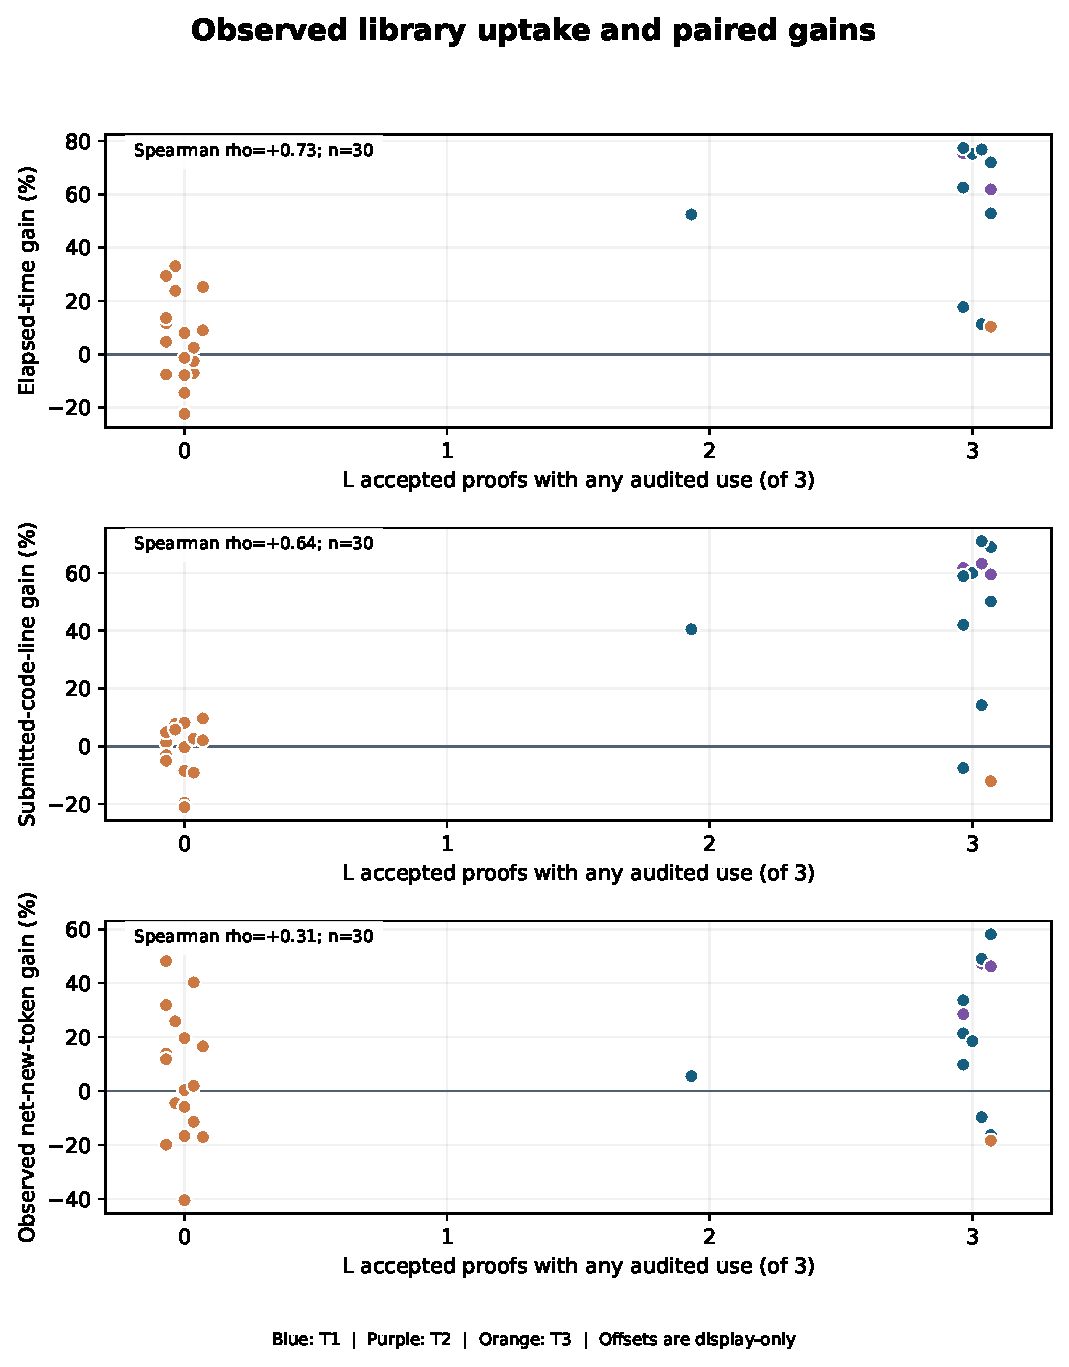
\includegraphics[width=\linewidth]{figures/uptake_gain.pdf}
\caption{Number of final L proofs with any dependency versus paired gains.
Colors identify prior expected tiers. Horizontal offsets are display-only;
the correlations are descriptive.}
\end{figure}

The three source/dependency scatter figures below use historical
expectation-tier colors, not outcome-based groups. The black ring marks
P15-T3, where direct proof-local helper use was present despite zero
archived target-distance-one reach. These figures are secondary diagnostics, not alternative
headline definitions of assistance. Their token panels use the same
observed net-new measure as the main figures.\footnote{
\pathref{make_extended_assets.py};
\pathref{../scope-sensitivity-30/scope_manifest.json}.}

\begin{center}\plot{qualified_distinct}\end{center}
\begin{center}\footnotesize\color{Muted}Distinct qualified source names; unqualified namespace-open uses can be missed.\end{center}
\clearpage
\begin{center}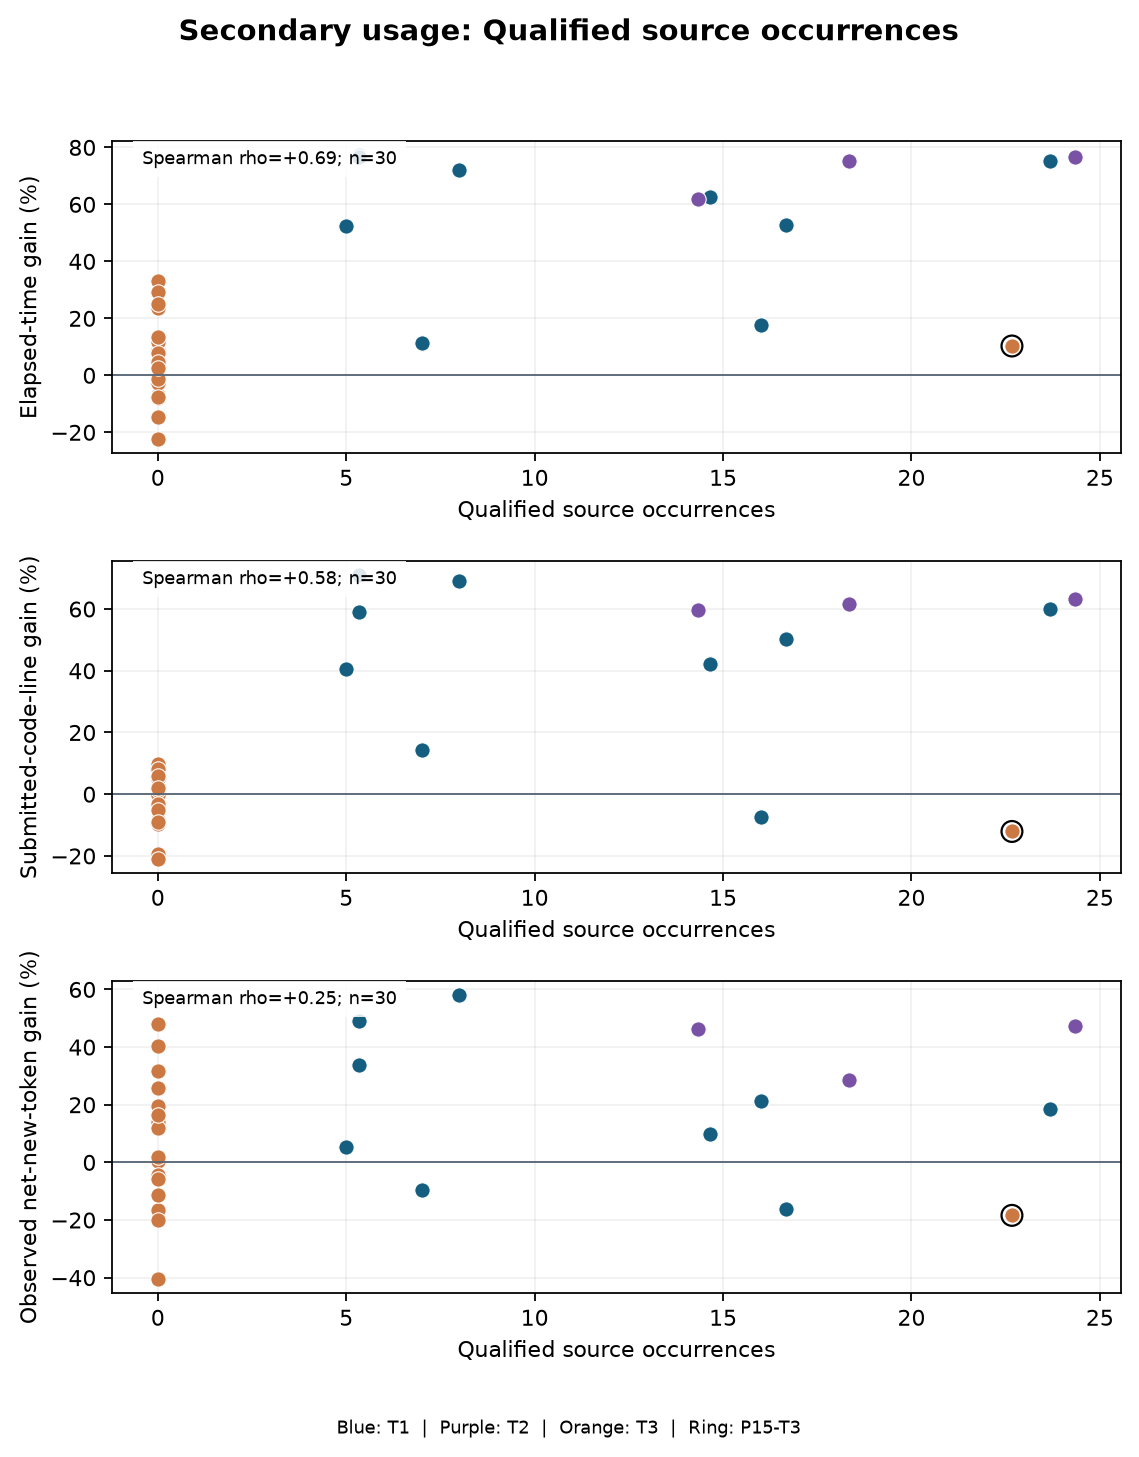
\includegraphics[width=\linewidth]{figures/qualified_occurrences.png}\end{center}
\begin{center}\footnotesize\color{Muted}Repeated qualified source occurrences; repeated spelling need not mean distinct mathematics.\end{center}
\clearpage
\begin{center}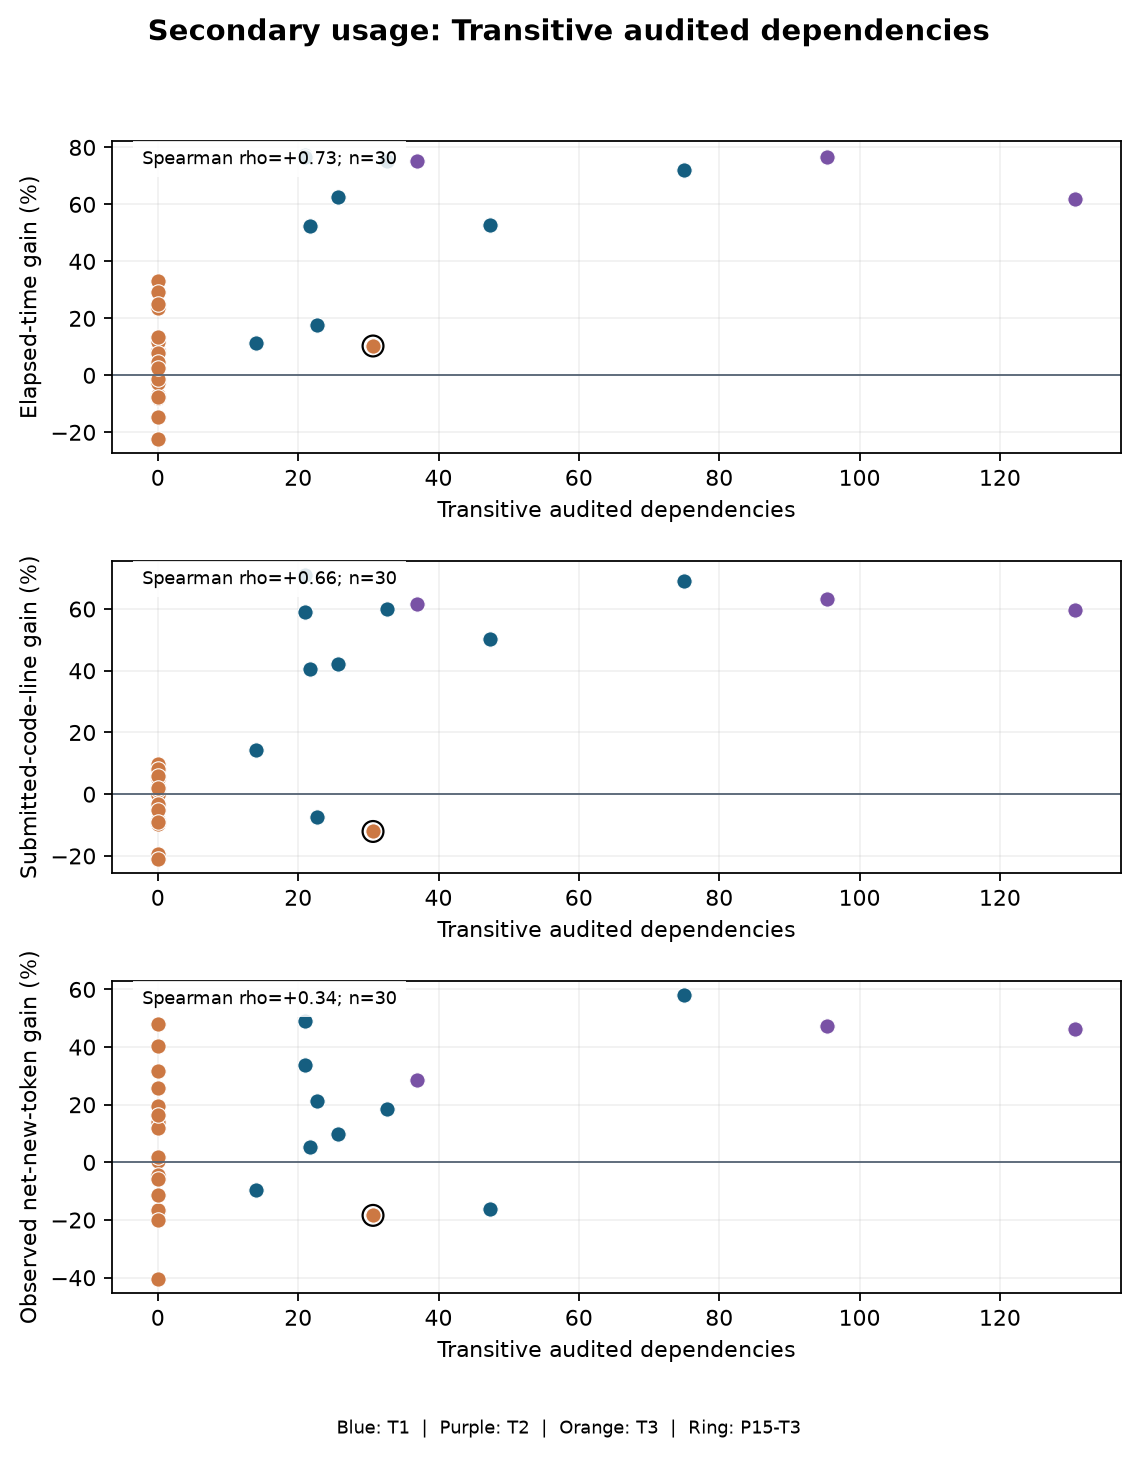
\includegraphics[width=\linewidth]{figures/transitive.png}\end{center}
\begin{center}\footnotesize\color{Muted}Transitive audited dependencies; indirect support and generated names enlarge the footprint.\end{center}

\begin{table}[htbp]\centering\small
\begin{tabular}{@{}lrrr@{}}\toprule
P01-T1 repetition & Any L dependency & Paired time gain & Paired physical-LOC gain \\\midrule
01 & no & -12.4\% & -24.8\% \\
02 & yes & +77.7\% & +53.5\% \\
03 & yes & +75.9\% & +75.0\% \\
\bottomrule

\end{tabular}
\caption{Three P01-T1 repetitions; the use choice was not assigned at
random. Two L repetitions with audited use averaged $+76.8\%$ time
and $+64.2\%$ LOC gain; the non-using repetition had $-12.4\%$
and $-24.8\%$. Three observations cannot establish a stable effect.
\pathref{../library-usage-analysis/mixed_task_usage.csv}.}
\end{table}

\clearpage
\section{Proof-region LOC diagnostic}\label{app:proofregion}
For each retained task, the table below gives the mean of three accepted
N and L target proof-region counts and their ratio-based gain. These
counts exclude pre-target helpers even when those helpers are needed
to complete the proof. They should not replace full submitted-file code
lines as the primary code-effort measure.\footnote{
\pathref{../library-usage-analysis/attempt_usage.csv},
\pathref{make_extended_assets.py}.}

\small
\begin{longtable}{@{}lrrr@{}}
\caption{Target proof-region nonblank, non-comment lines; positive
gain favors L. Complete submitted-file nonblank lines are in
Table~\ref{tab:tasks}.}\\
\toprule Task & N mean & L mean & Gain \\\midrule
\endfirsthead
\toprule Task & N mean & L mean & Gain \\\midrule
\endhead
P01-T1 & 33.3 & 39.7 & -19.0\% \\
P01-T2 & 4.3 & 19.0 & -338.5\% \\
P03-T3 & 258.3 & 273.0 & -5.7\% \\
P04-T1 & 105.0 & 139.0 & -32.4\% \\
P05-T3 & 61.7 & 96.3 & -56.2\% \\
P06-T3 & 78.0 & 82.3 & -5.6\% \\
P08-T3 & 175.7 & 44.7 & +74.6\% \\
P09-T3 & 57.0 & 91.7 & -60.8\% \\
P11-T3 & 219.3 & 201.7 & +8.1\% \\
P12-T1 & 68.7 & 54.0 & +21.4\% \\
P13-T3 & 187.7 & 178.0 & +5.2\% \\
P14-T1 & 102.3 & 133.0 & -30.0\% \\
P15-T1 & 15.3 & 32.3 & -110.9\% \\
P15-T2 & 65.7 & 114.3 & -74.1\% \\
P15-T3 & 25.7 & 230.3 & -797.4\% \\
P19-T3 & 260.7 & 189.0 & +27.5\% \\
P23-T1 & 125.7 & 156.7 & -24.7\% \\
P24-T3 & 90.7 & 89.3 & +1.5\% \\
P25-T3 & 41.0 & 59.0 & -43.9\% \\
P26-T1 & 80.7 & 74.7 & +7.4\% \\
P27-T3 & 62.3 & 59.3 & +4.8\% \\
P28-T1 & 57.3 & 56.7 & +1.2\% \\
P28-T3 & 170.7 & 156.0 & +8.6\% \\
P29-T1 & 30.3 & 35.7 & -17.6\% \\
P29-T2 & 55.3 & 91.3 & -65.1\% \\
P32-T3 & 77.7 & 44.0 & +43.3\% \\
P34-T3 & 132.7 & 120.0 & +9.5\% \\
P36-T3 & 33.0 & 37.3 & -13.1\% \\
P37-T3 & 20.0 & 54.7 & -173.3\% \\
P39-T3 & 124.7 & 121.7 & +2.4\% \\
\bottomrule

\end{longtable}
\normalsize

The historical physical-line measure, retained here for traceability,
includes blank and comment-only lines. It is not the line-counting rule
used for the main comparisons in either report.
\begin{longtable}{@{}lrrr@{}}
\caption{Historical complete-file physical lines; positive gain favors L.}\\
\toprule Task & N mean & L mean & Gain \\\midrule
\endfirsthead
\toprule Task & N mean & L mean & Gain \\\midrule
\endhead
P01-T1 & 137.7 & 83.7 & +39.2\% \\
P01-T2 & 311.0 & 124.3 & +60.0\% \\
P03-T3 & 317.3 & 319.0 & -0.5\% \\
P04-T1 & 430.3 & 371.0 & +13.8\% \\
P05-T3 & 632.7 & 568.7 & +10.1\% \\
P06-T3 & 349.7 & 346.0 & +1.0\% \\
P08-T3 & 676.7 & 631.7 & +6.7\% \\
P09-T3 & 2305.0 & 2513.3 & -9.0\% \\
P11-T3 & 353.0 & 344.0 & +2.5\% \\
P12-T1 & 253.7 & 129.0 & +49.1\% \\
P13-T3 & 331.0 & 341.7 & -3.2\% \\
P14-T1 & 233.7 & 250.7 & -7.3\% \\
P15-T1 & 264.7 & 108.0 & +59.2\% \\
P15-T2 & 727.3 & 270.7 & +62.8\% \\
P15-T3 & 730.3 & 810.7 & -11.0\% \\
P19-T3 & 427.7 & 440.7 & -3.0\% \\
P23-T1 & 439.3 & 259.0 & +41.0\% \\
P24-T3 & 113.7 & 136.3 & -19.9\% \\
P25-T3 & 116.3 & 127.0 & -9.2\% \\
P26-T1 & 539.7 & 174.3 & +67.7\% \\
P27-T3 & 203.7 & 192.3 & +5.6\% \\
P28-T1 & 259.7 & 111.7 & +57.0\% \\
P28-T3 & 190.3 & 171.0 & +10.2\% \\
P29-T1 & 240.7 & 74.0 & +69.3\% \\
P29-T2 & 993.7 & 412.3 & +58.5\% \\
P32-T3 & 165.3 & 169.3 & -2.4\% \\
P34-T3 & 214.3 & 203.3 & +5.1\% \\
P36-T3 & 119.7 & 145.3 & -21.4\% \\
P37-T3 & 226.7 & 245.7 & -8.4\% \\
P39-T3 & 157.7 & 149.3 & +5.3\% \\
\bottomrule

\end{longtable}

\section{Retained source-paper index}
The table maps every analyzed task to its paper identifier. Source titles and years come from \pathref{../../metadata/manifest.json}; current metadata establishes bibliography, not that an archived target equals a later redesigned one. Exact locators and paper hashes are recorded in the manifest and task artifacts.

\footnotesize\renewcommand{\arraystretch}{1.02}
\begin{longtable}{@{}lp{0.26\linewidth}p{0.62\linewidth}@{}}
\caption{All \ReportTasks\ retained archived task IDs and their \ReportPapers\ paper sources.}\\
\toprule
Paper & Archived task IDs & Source title and year \\\midrule
\endfirsthead
\toprule
Paper & Archived task IDs & Source title and year \\\midrule
\endhead
P01 & P01-T1, P01-T2 & The Accuracy of Floating Point Summation (1993) \\
P03 & P03-T3 & Accelerating the Solution of Linear Systems by Iterative Refinement in Three Precisions (2018) \\
P04 & P04-T1 & Mixed Precision Block Fused Multiply-Add: Error Analysis and Application to GPU Tensor Cores (2020) \\
P05 & P05-T3 & Improved Backward Error Bounds for LU and Cholesky Factorizations (2014) \\
P06 & P06-T3 & Probabilistic Rounding Error Analysis of Householder QR Factorization (2023) \\
P08 & P08-T3 & Iterative Refinement Implies Numerical Stability for Gaussian Elimination (1980) \\
P09 & P09-T3 & Roundoff Error Analysis of the Fast Fourier Transform (1971) \\
P11 & P11-T3 & A note on the error analysis of classical Gram-Schmidt (2006) \\
P12 & P12-T1 & A note on Dekker's FastTwoSum algorithm (2020) \\
P13 & P13-T3 & The numerical stability of barycentric Lagrange interpolation (2004) \\
P14 & P14-T1 & Accurately computing the log-sum-exp and softmax functions (2021) \\
P15 & P15-T1, P15-T2, P15-T3 & Solving block low-rank linear systems by LU factorization is numerically stable (2022) \\
P19 & P19-T3 & Mixed precision strategies for preconditioned GMRES: a comprehensive analysis (2026) \\
P23 & P23-T1 & Mixed-Precision Paterson-Stockmeyer Method for Evaluating Polynomials of Matrices (2025) \\
P24 & P24-T3 & Improving the Numerical Stability of Fast Matrix Multiplication (2016) \\
P25 & P25-T3 & A New Scaling and Squaring Algorithm for the Matrix Exponential (2009) \\
P26 & P26-T1 & Shifted Cholesky QR for Computing the QR Factorization of Ill-Conditioned Matrices (2020) \\
P27 & P27-T3 & Efficient Algorithms for Computing a Strong Rank-Revealing QR Factorization (1996) \\
P28 & P28-T1, P28-T3 & Backward Stability of Iterations for Computing the Polar Decomposition (2012) \\
P29 & P29-T1, P29-T2 & Accurate Symmetric Indefinite Linear Equation Solvers (1998) \\
P32 & P32-T3 & Backward Error and Condition of Structured Linear Systems (1992) \\
P34 & P34-T3 & Accurate Computations with Totally Nonnegative Matrices (2007) \\
P36 & P36-T3 & A Schur-Parlett Algorithm for Computing Matrix Functions (2003) \\
P37 & P37-T3 & Low Rank Solution of Lyapunov Equations (2002) \\
P39 & P39-T3 & Choosing the Forcing Terms in an Inexact Newton Method (1996) \\
\bottomrule

\end{longtable}
\normalsize\renewcommand{\arraystretch}{1.12}

\section{Evidence and regeneration index}
\begin{tabularx}{\linewidth}{@{}p{0.27\linewidth}X@{}}\toprule
Claim or artifact & Archived source \\\midrule
Retained task identity & \pathref{../scope-sensitivity-30/scope_manifest.json} and \pathref{retained_tasks.csv}; six-paper exclusion and 30 IDs. \\
Accepted attempts & \pathref{../library-usage-analysis/attempt_usage.csv}; source campaign, N/L pairing, proof paths and SHA-256, time, cached-inclusive archived token totals, physical and proof-region LOC, exact audited names. The aligned net-new derivation is \pathref{observed_net_new_tokens.json}. \\
Aggregated tasks & \pathref{../library-usage-analysis/task_usage.csv}; all 30 task means and paired gains. \\
Direct-proof use (DP) & \pathref{historical_direct_proof_scan.json}: 90 accepted L proof hashes, exact proof/local-helper declaration names, and counts. \pathref{historical_dp_manifest_v2.json} pins the archived proof, attempt, and common-definition hashes; \pathref{design33_proof_dependencies.lean} is the ten-task scanner. \\
Secondary target reach & Archived \pathref{../library-usage-analysis/attempt_usage.csv} fields \pathref{distance1_names} and \pathref{distance1_declarations}; task-level \pathref{mean_L_distance1} in \pathref{task_usage.csv}. This is not DP. \\
Historical protocols & \pathref{../../MEASUREMENT_PROGRESS.md}; r09/r10 replacement and r11 single-agent control. Individual \pathref{measurements/runs/results-r09/}, \pathref{results-r10/}, and \pathref{results-r11/} campaign locks and attempt records preserve effective prompt hashes and validation. \\
Environment & \pathref{measurements/runs/results-r11/environment/runtime_snapshot.json}, \pathref{resource_slots.json}, \pathref{host_at_creation.json}; software commits, slot ceilings, and hardware inventory. \\
Report data and figures & \pathref{build_data.py}, \pathref{token_measurement.py}, \pathref{rescan_historical_dp.py}, and \pathref{make_extended_assets.py}; \pathref{report_data.json}, \pathref{observed_net_new_tokens.json}, \pathref{extended_stats.json}, \pathref{accepted_code_line_scan.json}, generated \pathref{tables/} and \pathref{figures/}. \\
\bottomrule\end{tabularx}

The plotted and tabulated report can be regenerated from the archived
ledgers by running \pathref{build_data.py} followed by
\pathref{make_extended_assets.py}, then compiling this LaTeX file.
Re-running the historical
\emph{contestants} is a different operation: it requires the frozen
campaign controller, exact runtime snapshots, provider access, and
effective prompts. This report is not evidence of such a fresh rerun.

\end{document}
